\chapter{Fonctions réelles et continuité}
\section{Introduction}

\begin{boxdef}[Fonction réelle]
Soit $D \subseteq \mathbb{R}$ un ensemble de nombres réels. Une \emph{fonction réelle} $f : D \to \mathbb{R}$ est un procédé qui associe à chaque nombre $x \in D$ un unique nombre réel $y \in \mathbb{R}$, que l'on note $y = f(x)$.

On appelle $D$ l'\emph{ensemble de définition} de $f$.
\end{boxdef}
Par exemple, la fonction $f : \mathbb{R} \to \mathbb{R}$ définie par $f(x) = 2x$ est la fonction qui associe à chaque $x \in \mathbb{R}$ son double. Son ensemble de définition est $\mathbb{R}$ tout entier, car elle est bien définie pour chaque nombre réel. Ce n'est pas le cas de toutes les fonctions que vous avez rencontré~: la fonction $g$ définie par $g(x) = \frac{1}{x}$ qui associe à chaque $x$ son \emph{inverse multiplicatif} n'est pas défini en $x = 0$, car la division par 0 est une opération indéfinie. En effet, puisque la division est définie comme la réciproque de la multiplication, diviser $1$ par $x$ revient à chercher le nombre $y \in \mathbb{R}$ tel que $xy = 1$. Or, pour $x = 0$, on obtient la contradiction $0\cdot y = 0 = 1$, ce qui n'est vrai pour aucun $y$.

Puisque les fonctions associent à chaque $x \in D$ un unique $y = f(x) \in \mathbb{R}$, on peut les représenter par un \emph{graphe} sur un plan cartésien 2-dimensionnel, où l'on affiche les points de coordonnées $(x, f(x))$. Pour les deux fonctions $f$ et $g$ ci-dessus, on obtient les \emph{graphes} suivants~:
\begin{figure}[H]
    \centering
    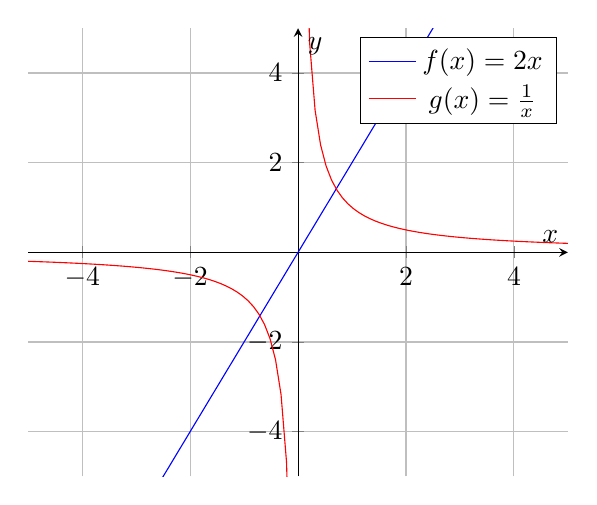
\begin{tikzpicture}
        \begin{axis}[
            xmin = -5,
            ymin = -5,
            xmax = 5,
            ymax = 5,
            xlabel = $x$,
            ylabel = $y$,
            axis lines = middle,
            grid
        ]
        
        \addplot[blue, domain=-5:5] {2 * x};
        \addlegendentry{$f(x) = 2x$};
        
        \addplot[red, domain=-5:-0.01, samples = 50] {1 / x};
        \addplot[red, domain=0.01:5, samples = 50] {1 / x};
        \addlegendentry{$g(x) = \frac{1}{x}$};
        
        \end{axis}
    \end{tikzpicture}
    \caption{Graphes des fonctions $f(x) = 2x$ et $g(x) = \frac{1}{x}$}
    \label{fig:graph_basic_functions}
\end{figure}

Gardons en tête ces deux graphes. Observons d'abord qu'ils permettent de visualiser assez facilement les propriétés de nos deux fonctions, en particulier la singularité de $g$ en 0. Il devient alors évident par le graphe qu'il est impossible de définir naturellement la division par $0$.

En outre, on pourrait dire que $f$ est \emph{plus régulière} que $g$, dans le sens où elle n'admet pas de point problématique, i.e. elle n'admet pas de saut. C'est cette intuition là que l'on cherchera à développer d'une manière plus systématique dans les prochaines sections, en cherchant ce qui fait de $f$ une "meilleure" fonction que $g$.

\section{Limite de fonction}
\subsection{Limite à droite, limite à gauche}
Le Graphe \ref{fig:graph_basic_functions} de $g$ permet de voir assez facilement le comportement de la fonction autour de $0$. En effet, du côté négatif, les valeurs de $g$ sont négativement de plus en plus grandes, à mesure que l'on s'approche de 0 de la gauche. D'une manière symétrique, les valeurs de $g$ du côté positif croissent lorsque l'on s'approche de 0 de la droite. De plus, il semblerait que cette croissance soit \emph{non-bornée}, i.e. on peut trouver des valeurs arbitrairement grandes. Pour s'en convaincre, on peut écrire certaines valeurs de $g(x)$ autour de 0 du côté positif~:
\begin{table}[H]
    \centering
    \begin{tabular}{|c|c|}
        \hline
        $x$ & $g(x)$ \\
        \hline
        $0.1$ & $\frac{1}{0.1} = 10$ \\
        \hline
        $0.01$ & $\frac{1}{0.01} = 100$ \\
        \hline
        $\vdots$ & $\vdots$ \\
        \hline
        $10^{-50}$ & $10^{50}$ \\
        \hline
        $\vdots$ & $\vdots$ \\
        \hline
    \end{tabular}
    \caption{Table des valeurs de $g(x)$ quand $x \to 0$, $x > 0$}
    \label{tab:singularity_values}
\end{table}
On a alors envie d'écrire par unicité que la limite de $g(x)$ quand $x \to 0$ est $\infty$, i.e. $\displaystyle\lim_{x \to 0} g(x) = \infty$. Pourtant, lorsque l'on approche 0 du côté négatif, on a manifestement une limite différente, à savoir $-\infty$. Ainsi, que l'on approche $0$ de la droite ou de la gauche, on obtient deux résultats qui ne sont pas nécessairement égaux. Ces deux manières d'approcher un point sont matérialisées dans les notions de \emph{limite à droite} et \emph{limite à gauche} d'une fonction~: on voit à partir de notre graphe que les limites à droite et à gauche de $g$ en $0$ sont
\begin{equation}
\lim_{x \to 0^{-}} \frac{1}{x} = -\infty \quad \mathrm{ et } \quad \lim_{x \to 0^{+}} \frac{1}{x} = \infty
\end{equation}
où les notations $0^{-}$ et $0^{+}$ désignent le côté où l'on approche $0$.

Observons que les limites à droite et à gauche nous permettent de définir ce que l'on entendait par un "saut"~: une fonction n'a pas de saut en un point si les limites à droite et à gauche en ce point coïncident. Dans ce cas, on peut parler sans ambiguïté de \emph{la} limite en ce point, sans préciser le côté par lequel on approche la limite, et on la définit comme le résultat des deux limites.

Les limites de fonctions partagent de nombreuses similarités avec les limites de suites, que l'on a introduit dans le Chapitre \ref{chap:suite}. En particulier, on peut appliquer les propriétés de linéarité et le théorème des gendarmes, de la même manière que si l'on traitait avec des suites.

\subsection{Continuité}
En réalité, il existe plusieurs autres manières moins évidentes pour qu'une fonction admette un saut en un point. Elle peut ne pas être définie en ce point mais tout autour, ce qui cause un saut dans le domaine de définition. Il se peut aussi que la fonction soit définie en ce point, mais que les limites à droite et à gauche ne soient pas égales à cette valeur. C'est le cas de notre fonction $f$, si on change une valeur en un point, par exemple en définissant la fonction $\hat{f}(x) = \begin{cases} f(x) = 2x & \textrm{si } x \neq 1 \\ 1 & \textrm{si } x = 1 \end{cases}$.
Ainsi, 
\begin{equation}
\lim_{x \to 1} \hat{f}(x) = \lim_{x \to 1} 2x = 2 \neq \hat{f}(1) = 1
\end{equation}
et la fonction $\hat{f}$ saute lorsqu'elle arrive à 1, ce que l'on peut distinguer sur la Figure ci-dessous~:
\begin{figure}[H]
    \centering
    \begin{tikzpicture}
        \begin{axis}[
            xmin = -2,
            ymin = -5,
            xmax = 4,
            ymax = 5,
            xlabel = $x$,
            ylabel = $y$,
            axis lines = middle,
            grid,
            legend style={font=\tiny,cells={align=right}}
        ]
        
        \addplot[orange, domain=-2:0.99] {2 * x};
        \addplot[orange, domain=0.99:4] {2 * x};
        \addlegendentry{$\hat{f}(x) = \begin{cases} 2x & \textrm{si } x \neq 1 \\ 1 & \textrm{si } x = 1 \end{cases}$\\};
        
        \addplot[color=orange,fill=white,only marks,mark=*] coordinates{(1,1)};
        \draw[dotted,orange] (axis cs:1,1) -- (axis cs:1,2);
        
        \end{axis}
    \end{tikzpicture}
    \caption{Graphe de la fonction $\hat{f}$}
    \label{fig:function_jump}
\end{figure}

On définit ainsi la notion primordiale de \textbf{continuité} d'une fonction dans le fait qu'elle n'admette pas de saut, comme décrit ci-dessus~:
\begin{boxdef}[Continuité]\label{def:continuité}
Soit $f : D \to \mathbb{R}$ une fonction réelle, $a \in \mathbb{R}$ un nombre réel. On dit que $f$ est \emph{continue} en $a$ si
\begin{enumerate}
    \item Les limites à droite et à gauche existent et sont égales, i.e.
    \begin{equation}
    \lim_{x \to a^+} f(x) = \lim_{x \to a^-} f(x) \eqdef \lim_{x \to a} f(x) \in \mathbb{R}
    \end{equation}
    
    \item $f$ est définie en $a$, i.e. $a \in D$.
    
    \item La limite de $f$ en $a$ est égale à $f(a)$, i.e.
    \begin{equation}
    \lim_{x \to a} f(x) = f(a)
    \end{equation}
\end{enumerate}
On dit d'une manière similaire que $f$ est continue sur $E \subseteq D$ si $f$ est continue en tout point de $E$. (Si $D = E$, on omet généralement de mentioner $E$, et on dit simplement que $f$ est une fonction continue).
\end{boxdef}
Prenez un moment pour vous convaincre que chacun des 3 points de la définition est important dans la définition de la continuité. Le premier garantit que les voisinages à droite et à gauche du point sont au même niveau, le deuxième garantit qu'il n'y ait pas de saut horizontal dans le domaine de définition, et le dernier garantit qu'il n'y a pas de saut en le point lui-même.

La plupart des fonctions élémentaires que vous pouvez imaginer, telles que les polynômes, les fonctions trigonométriques, exponentielles, logarithmiques, etc. sont continues. De plus, la somme, le produit, le quotient et la composition de fonction continues sont des fonctions continues, ce qui permet aisément de déterminer si une fonction est continue à partir de fonction connues. Plus précisément~:
\begin{boxthm}[Propriétés des fonctions continues]
Soit $f, g$ deux fonctions réelles continues en $x \in \mathbb{R}$. Alors~:
\begin{enumerate}
    \item $f + g$ est continue en $x$.
    \item $f \cdot g$ est continue en $x$.
    \item Si $g(x) \neq 0$, $\frac{f}{g}$ est continue en $x$.
    \item Si $g$ est continue en $f(x)$, alors $g \circ f$\footnote{$g \circ f : \mathbb{R} \to \mathbb{R}$ est la fonction \emph{composée} de $f$ par $g$, définie par $(g \circ f)(x) = g(f(x))$, c'est-à-dire l'application de la fonction $f$ suivie de $g$.} est continue en $x$.
\end{enumerate}
\end{boxthm}

\subsection{Prolongement par continuité}
Considérons la fonction $s(x) = \frac{\sin(x)}{x}$\footnote{Culture générale~: on appelle parfois cette fonction \emph{sinus cardinal}, et on la note $\mathrm{sinc}$}, définie en tout point de $\mathbb{R}$ sauf en 0. Pour bien comprendre son comportement, prenons son graphe autour de 0~:
\begin{figure}[H]
    \centering
    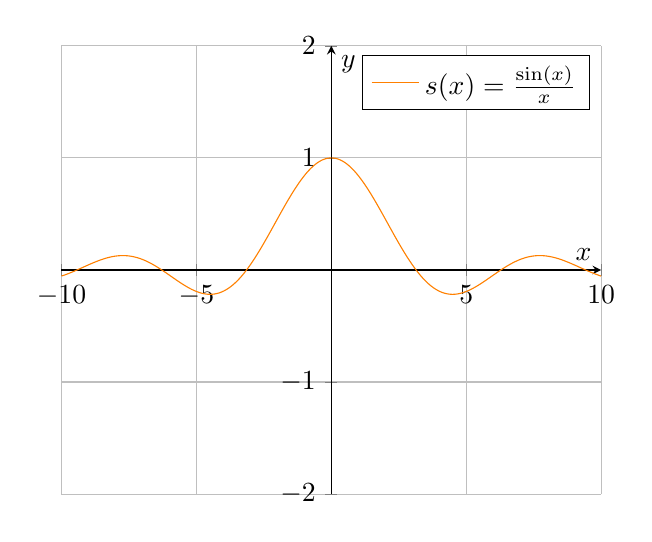
\begin{tikzpicture}
        \begin{axis}[
            xmin = -10,
            ymin = -2,
            xmax = 10,
            ymax = 2,
            xlabel = $x$,
            ylabel = $y$,
            axis lines = middle,
            grid,
            trig format plots=rad
        ]
        
        \addplot[orange, domain=-10:-0.01,samples=300] {sin(x) / x};
        \addplot[orange, domain=0.01:10,samples=300] {sin(x) / x};
        \addlegendentry{$s(x) = \frac{\sin(x)}{x}$};
        
        \end{axis}
    \end{tikzpicture}
    \caption{Graphe de la fonction $s(x) = \frac{\sin(x)}{x}$}
    \label{fig:sin_over_x}
\end{figure}
Notre fonction satisfait manifestement la première contrainte de notre Définition \ref{def:continuité}, car les limites à droite et à gauche sont égales à 1, tandis qu'elle n'est pas définie en 0. Il est possible dans ce cas de la \emph{prolonger} en une fonction continue, que l'on note avec un tilde~:
\begin{equation}
\tilde{s}(x) = \begin{cases}
s(x) = \frac{\sin(x)}{x} & \textrm{si } x \neq 0 \\
1 & \textrm{si } x = 0
\end{cases}
\end{equation}
Ainsi, $\tilde{s}$ est définie en 0, et
\begin{equation}
\lim_{x \to 0^{-}} \tilde{s}(x) = \lim_{x \to 0^{+}} \tilde{s}(x) = \lim_{x \to 0} \tilde{s}(x) = 1 = \tilde{s}(0)
\end{equation}
Donc $\tilde{s}$ est bien continue en 0 (même sur tout $\mathbb{R}$). Ce procédé de transformation d'une fonction $f$ autour d'un point problématique $a$ en une fonction continue en $a$ est appelé le \emph{prolongement par continuité} de $f$ en $a$. Notons que cette transformation est valide que si la limite existait, c'est-à-dire que le premier point doit être validé au préalable.

\begin{greybox}
\textit{Et alors ? Pourquoi c'est si important cette histoire de continuité ?}
\end{greybox}

Eh bien, la continuité a de nombreuses conséquences sur le comportement de notre fonction. Cela assure une certaine régularité locale autour d'un point, ou même plus globale si la fonction est continue sur tout son ensemble de définition. C'est ces théorèmes que l'on va aborder dans la fin de ce chapitre.

\section{Théorème de la valeur intermédiaire}
Le théorème de la valeur intermédiaire est l'un des résultats majeurs qui porte sur les fonctions continues. Il énonce que la continuité telle que nous l'avons définie respecte bien nos attentes, à savoir qu'il n'y a pas de saut dans une fonction continue sur un intervalle. Plus précisément~:
\begin{boxthm}[Théorème de la valeur intermédiaire]
Soit $f : D \to \mathbb{R}$ une fonction continue, $I = [a, b] \subseteq D$ un intervalle réel. Alors l'image de $[a, b]$ par $f$ est un intervalle, c'est-à-dire que $f$ prend toutes les valeurs entre son minimum et son maximum sur l'intervalle~:
\begin{equation}
f([a, b]) = \left[\min_{x \in [a, b]} f(x), \max_{x \in [a, b]} f(x)\right]
\end{equation}
où $f([a, b])$ désigne l'ensemble des valeurs de $f$ sur l'intervalle $[a, b]$.
\end{boxthm}
Par exemple, la fonction $h(x) = e^x + x$ est une fonction croissante et continue sur $[0, 1]$, par somme de fonction continues. Ainsi, le théorème ci-dessus implique que sur l'intervalle $[0, 1]$, $f$ atteint son minimum $h(0) = 1$, son maximum $h(1) = e + 1$, et \emph{tout nombre réel intermédiaire} entre $1$ et $e + 1$. Il nous permet e.g. d'affirmer qu'il existe un $c \in [a, b]$ tel que $h(c) = e$, car $1 \leq e \leq e + 1$.

Un cas particulier arrive lorsque $f$ est une fonction telle que $f(a) \leq 0$ et $f(b) \geq 0$. Dans ce cas, on peut affirmer qu'il existe une solution $c \in [a, b]$ à l'équation $f(c) = 0$, ce qui est l'objet du corollaire suivant~:
\begin{boxcorollary}
Soit $f : D \to \mathbb{R}$ une fonction continue sur un intervalle $I = [a, b] \subseteq D$, avec $f(a) \leq 0$ et $f(b) \geq 0$. Alors il existe $c \in [a, b]$ tel que
$f(c) = 0$.
\end{boxcorollary}
Par exemple, pour notre fonction $h$ ci-dessus, observons que
\begin{equation}
h(-1) = e^{-1} - 1 \approx -0.63 \quad \textrm{et} \quad h(0) = e^0 = 1
\end{equation}
Ainsi, on sait qu'il existe un nombre $x_0 \in ]-1, 0[$ tel que $e^{x_0} + x_0 = 0$. En fait, en rapprochant les bornes de l'intervalle, on peut approximer numériquement la valeur de $x_0$ à une précision arbitraire, et ce malgré le fait qu'il soit impossible de trouver la solution de l'équation de manière algébrique (on dit que la solution n'est pas \emph{analytique}). Ce théorème nous permet donc par une étude minutieuse de trouver le nombre de solutions d'une équation faisant intervenir des fonctions continues.